This section is intended to make the developer understand the working of the Colletta frontend, and to allow him or her to add functionalities  to the software package.
In order fully understand the contents below, the developer must have a certain degree of familiarity with React and Redux. If that's not the case, we strongly recommend the reader to at least acquire some basic knowledge on the topics.
\subsection{Frontend UML}
To help a better comprehension of the front-end architecture we created the following figure:
\begin{figure}
\centering 
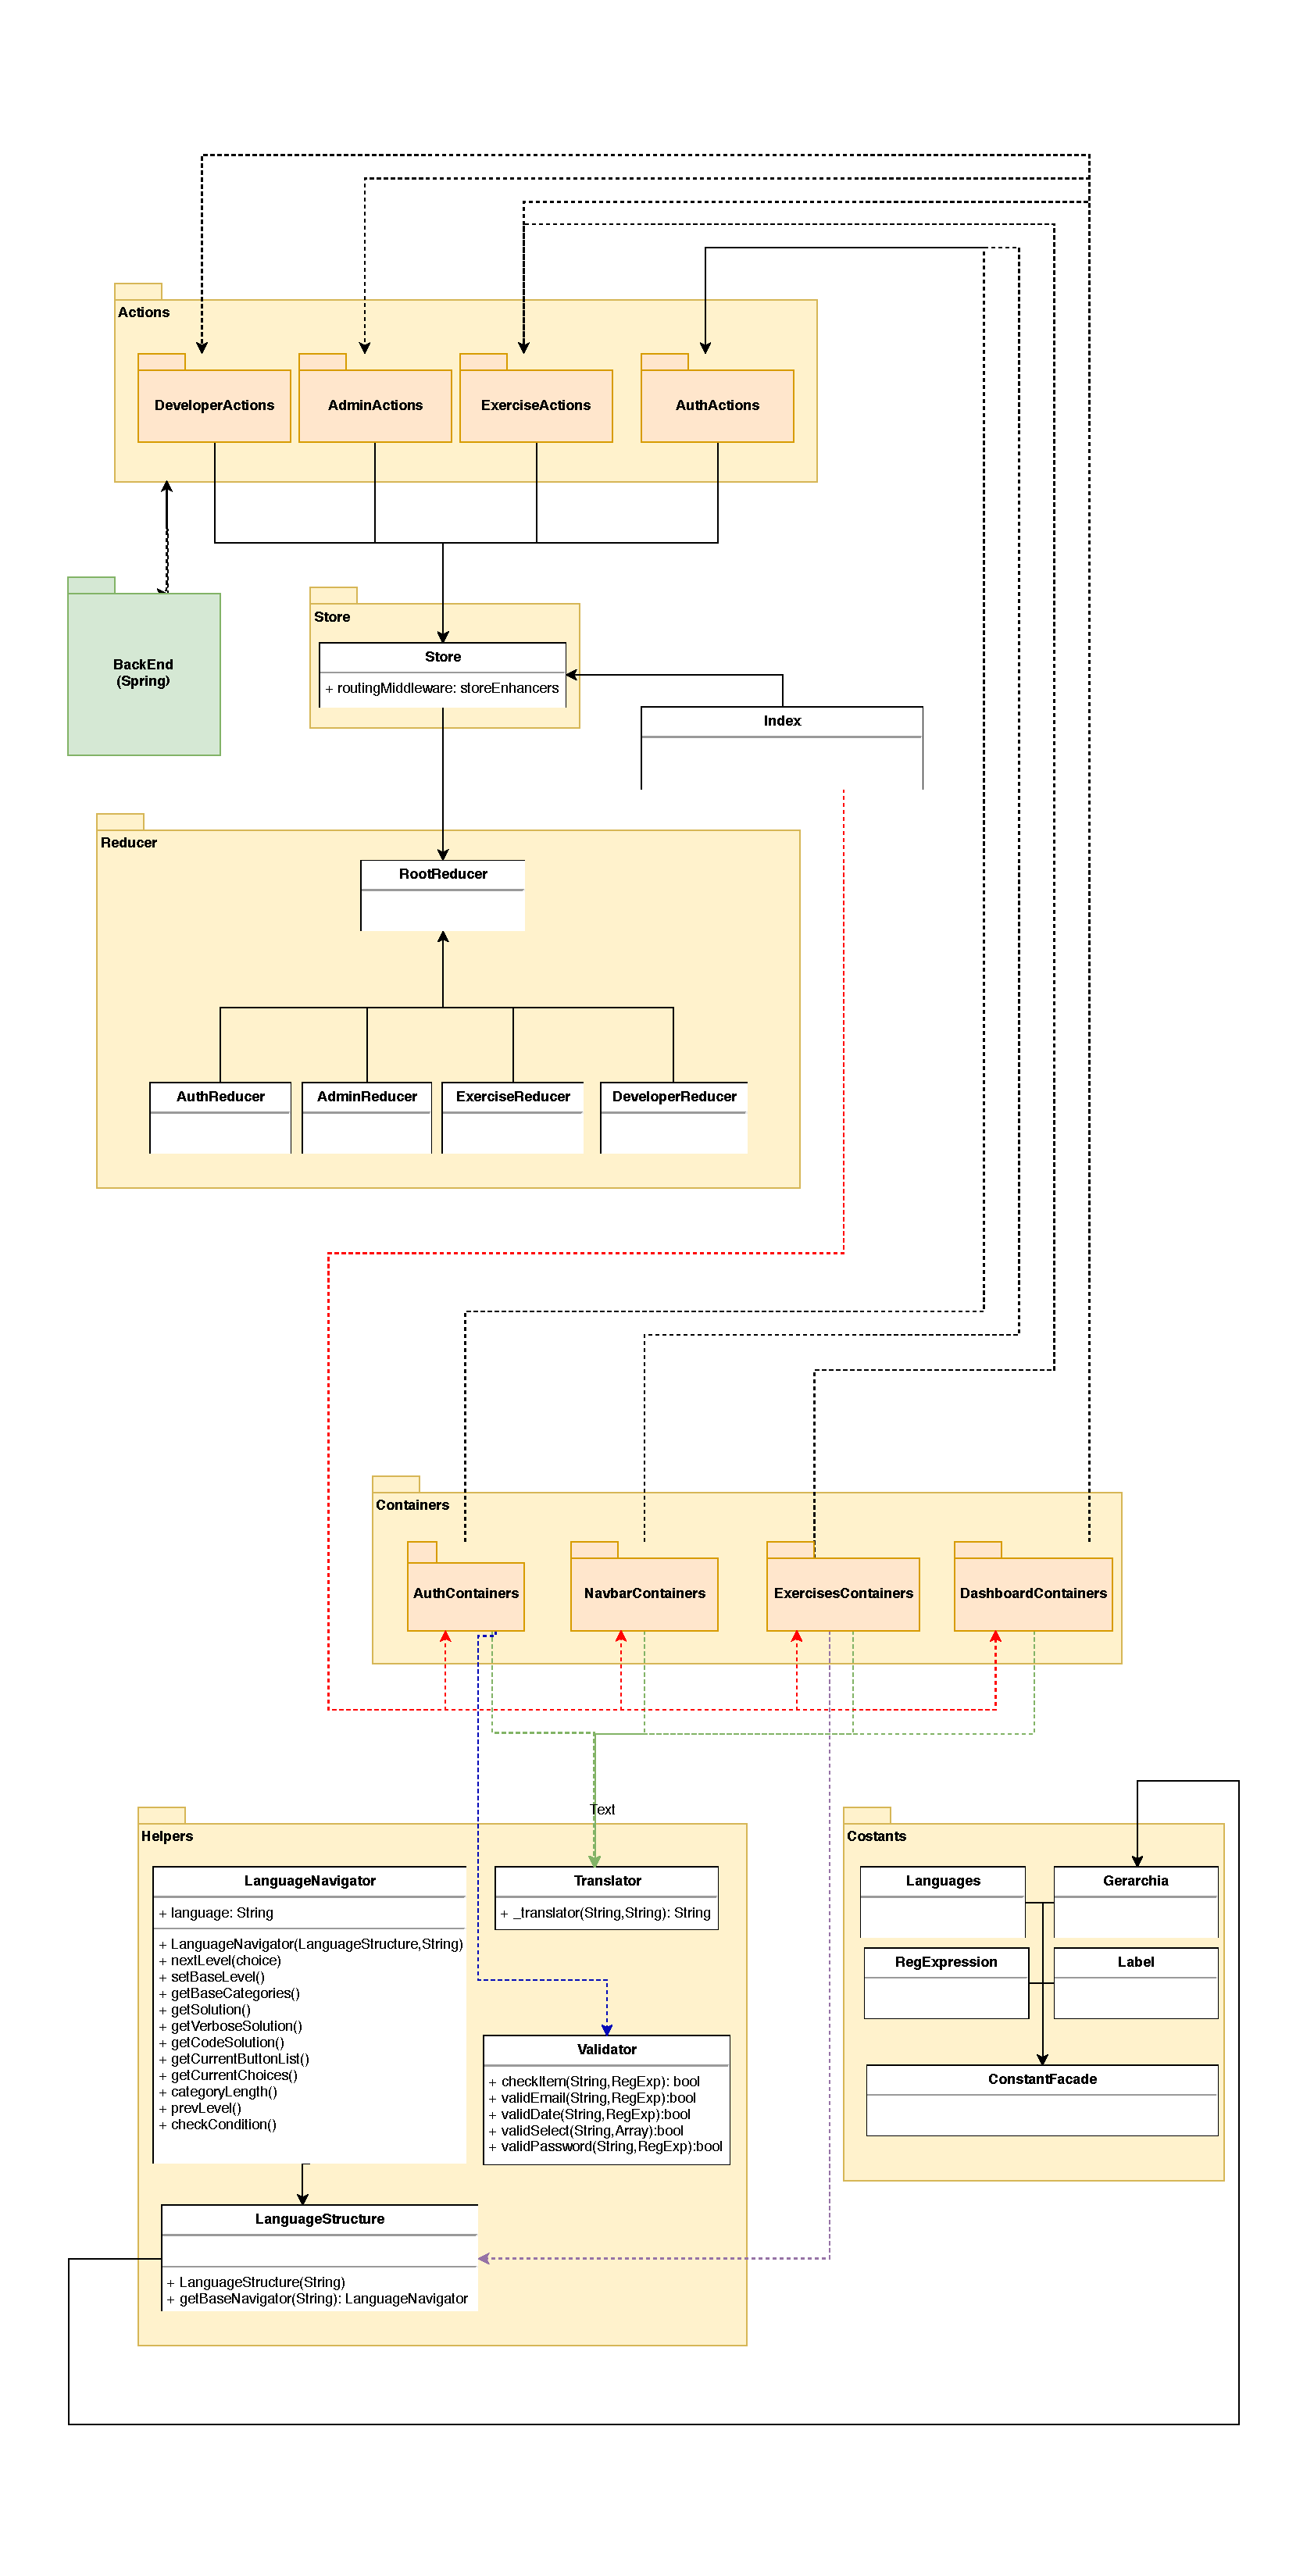
\includegraphics[width=15cm, height=18cm]{uml/reactredux.pdf} 
\caption{React and Redux architecture}
\end{figure}
\subsection{Directory tree}
\begin{figure}[H]
\centering
\begin{forest}
  for tree={
    font=\ttfamily,
    grow'=0,
    child anchor=west,
    parent anchor=south,
    anchor=west,
    calign=first,
    inner xsep=7pt,
    edge path={
      \noexpand\path [draw, \forestoption{edge}]
      (!u.south west) +(7.5pt,0) |- (.child anchor) pic {folder} \forestoption{edge label};
    },
    before typesetting nodes={
      if n=1
        {insert before={[,phantom]}}
        {}
    },
    fit=band,
    before computing xy={l=15pt},
  }  
[Frontend
	[src
		[actions
		]
		[assets
		]
		[constants
		]
		[helpers
		]
		[reducer
		]
		[store
		]
		[view
			[containers]
			[components]
		]
	]
]
\end{forest}
\caption{Frontend directory tree}
\label{fig:BackDir}
\end{figure}

Each folder contains a specific set of files:
\begin{itemize}
	\item \textbf{actions:} the modules in this folder are responsible for creating and dispatching the actions to the reducers;
	\item \textbf{assets:} static files like font and images;
	\item \textbf{constants:} data collections and constants used in various part of the code, i.e. the label used for the translation;
	\item \textbf{helpers:} standard js functions or classes which have some use in the code, i.e. the label translator;
	\item \textbf{reducers:} all the reducers responsible for the creation of a new state;
	\item \textbf{store:} a single file creating and giving access to the centralized state;
	\item \textbf{view:} classes rendering the information in the store. They are divided in \textit{components} and \textit{containers}.	 The key point to bare in mind when talking about components and containers is the following: containers are "smart", they observe the store and can call actions; components, on the other hand, are basically just static functions.
\end{itemize}

\subsection{Modify or add features}
\subsubsection{Components}
Components extend the React \texttt{component} abstract class and implement the \texttt{render()} method. They can be viewed as a pure functions of the props passed by their father component or container. They do not have access to the store. When adding or modifying a component the following rules should be followed:
\begin{itemize}
	\item Since the global state of the application is managed by Redux, do not use or create the local state of the component. Instead, rely solely on the props;
	\item Helper functions may be defined in the component class, but none of them should call action creators or external resources such as API calls;
	\item All components must be placed in the \texttt{src/component} folder;
	\item Every component which needs to render some text must have a language prop to call to the translator module;
\end{itemize}
When adding a new component, one can start from the following snippet:
\begin{lstlisting}[language=JavaScript, frame=single]
import React, { Component } from 'react';
import _translator from '../../helpers/Translator';
class SampleComponent extends Component {

  render() {
    const { prop1,prop2,prop3 } = this.props;
    //Do stuff here
    return (
      <React.Fragment>
        {/* Stuff to render */}
      </React.Fragment>
    );
  }
}
export default SampleComponent;
\end{lstlisting}


\subsubsection{Containers}
Containers extend the React \texttt{component} abstract class and implement the \texttt{render()} method. They can read the store and alters its state via actions. Containers can also have props passed to them, just like a container. When adding or modifying a component the following rules should be followed:
\begin{itemize}
	\item Since the global state of the application is managed by Redux, do not use or create the local state of the container. Instead, rely solely on the props and on the store;
	\item The store and the actions should not be accessed directly for performance and readability reasons. Instead, the should be mapped to the props;
	\item All containers must be placed in the most appropriate \texttt{src/view/containers} sub-directory. Creation of new sub-directories is allowed if necessary.
\end{itemize}

When adding a new container, one can start from the following snippet:
\begin{lstlisting}[language=JavaScript, frame=single]
import React, { Component } from 'react';
import { connect } from 'react-redux';
import _translator from '../../../helpers/Translator';

class SampleContainer extends Component {

  render() {
    const { prop1, prop2, prop3, action1Prop, action2Prop } = this.props;
    // Do stuff
    return (
      // Stuff to render
    );
  }
}
const mapStateToProps = store => {
  return {
    prop1: store.object1,
    prop2: store.object2,
    prop3: store.object3
  };
};

const mapDispatchToProps = dispatch => {
  return {
    action1Prop: () => dispatch(action1()),
    action2Prop: () => dispatch(action2())
  };
};
//both action1 and action2 must be imported

export default connect(
  mapStateToProps,
  mapDispatchToProps
)(SampleContainer);
\end{lstlisting}


\subsubsection{Rest API calls}
When implementing a new Rest API call (RAP from now on), the developer must stick to the following guidelines:
\begin{itemize}
	\item RAPs must be implemented inside an action creator and should not be put inside components or containers;
	\item RAPs must use the Axios module;
	\item RAPs must pass an authorization token (exception made for Login and SignUp) which is kept in the store. The snippet below will show clarify how;
	\item If a RAP does not need additional data, the data field should be replaced by \texttt{\{\}}, otherwise the response will display a 403 error.
\end{itemize}
When adding a new RAP, one can start from the following snippet:
\begin{lstlisting}[language=JavaScript, frame=single]
export const sampleActionCreator = objectToSend => {
  return dispatch => {
    axios
      .post(
        'http://localhost:8081/sample-call',
        {
          ...objectToSend
        },
        {
          headers: {
            'content-type': 'application/json',
            Authorization: store.getState().auth.token
          }
        }
      )
      .then(response => {
        // Maybe do something
        dispatch({ type: 'SAMPLE-ACTION', dataToDispatch });
      })
      .catch(() => {/* Handle Error Here*/});
  };
};
\end{lstlisting}


\subsubsection{Interface Language}
The multiple languages of the application are implemented via the Translator module in the \texttt{src/helpers} folder. Every single piece of text shown to the user is stored in \texttt{src/constants/Label.js} in all the languages supported by Colletta. Each language is identified by its ISO 639-1 code.\\
Each string variable is composed as follow:
\begin{center}
context\_identifier
\end{center}
where:
\begin{itemize}
\item \textbf{Context} is the component or container in which the string is used. If it is used in more than one component or container, context should be \texttt{gen}. Context must start with a lowercase letter;
\item \textbf{Identifier} should sum up the function of the string. It must start with a lowercase letter.
\end{itemize}
The translated string can than be displayed with the following function:
\begin{center}
\texttt{\_translator('string\_variable', language)}
\end{center}
where:
\begin{itemize}
\item \textbf{String\_variable} is the name of the string you want to render. It must be surrounded by single quotes;
\item \textbf{Language} is a string containing the ISO 639-1 code of the language you want to render the string in.
\end{itemize}
Therefore, whenever one wants to add some new text to some component or container, he or she must add the string in all of the supported languages and render it with the translator module.\\
If instead one wants to implement a new language, the following steps need to followed:
\begin{enumerate}
\item Every single string in \texttt{Label.js} must be translated and inserted with the ISO 639-1 code of the language;
\item The variable \texttt{UiLang} in \texttt{src/constants/Label.js} must be updated with the ISO 639-1 code of the language;
\item For every language in \texttt{Label.js}, a string int the format \texttt{gen\_xx} must be added, with xx being the ISO 639-1 code of the language. The string must contain the language name. For instance, in English \texttt{gen\_it} is Italian and \texttt{gen\_en} is English.
\end{enumerate}
The following snippet represents a slim-down example of \texttt{Label.js}:
\begin{lstlisting}[language=JavaScript, frame=single]
export const _label = {
  it: {
    account_yourData: 'I tuoi dati',
    dashboard_hiUser: 'Ciao, ',
    executionExercise_complete: 'Completa',
    gen_it: 'Italiano',
    gen_en: 'Inglese'
  },
  en: {
    account_yourData: 'Your data',
    dashboard_hiUser: 'Hello, ',
    executionExercise_complete: 'Submit solution',
    gen_it: 'Italian',
    gen_en: 'English',
  }
};
\end{lstlisting}


\subsubsection{Analysis Languages}
The process for enabling other analysis language is a little bit more tedious, as it means having to do with the Freeling tagset.
Let's have a brief overview at what needs to be done:
\begin{enumerate}
\item A custom JSON tagset must be created starting from the freeling tagset;
\item The tagset created must be modified to accommodate some conditions;
\item The tagset must be placed in the correct folder.
\end{enumerate}
One can find the Freeling tagsets and their description at: \href{https://talp-upc.gitbook.io/freeling-4-1-user-manual/tagsets}{freeling-4-1-user-manual}. Starting from the tables in the Freelig doc, the end result should look like this:
\begin{lstlisting}[language=JavaScript, frame=single]
const italian = {
  adjective: {
    text: { full: 'adjective', short: 'A' },
    attributes: [
      {
        attrName: 'type',
        choices: [
          { short: 'O', full: 'Ordinal' },
          { short: 'Q', full: 'qualificative' },
          { short: 'P', full: 'Possesive' }
        ],
        condition: null
      },
      {
        attrName: 'degree',
        choices: [
          { short: 'S', full: 'superlative' },
          { short: '0', full: 'none' }
        ],
        condition: { index: 1, short: 'Q' }
      },
      //...........
\end{lstlisting}
Let's break in down:
\begin{itemize}
\item The outermost level contains the categories of word in the language (i.e. adjective, noun, etc...);
\item Each category has a text value, a name, a condition, and a list of choices. Each choice represents a possible value for the attribute.
\item Choices and text objects of attributes contain two string:
	\begin{itemize}
	\item \textbf{Full:} the name of the choice or category (i.e. Adjective, Ordinal).
	\item \textbf{Short:} the letter corresponding to the choice or the category (i.e. Adjective is A, Ordinal is O.
	\end{itemize}
\end{itemize}
The modifications which have been made from the standard tagset are the following:
\begin{itemize}
\item \textbf{Conditions}: this field is needed for avoiding showing the user choices that cannot be taken. For instance, it would make non sense to show the option to show the superlative option if the adjective selected has been marked as possessive. Thus, the condition states that the attribute at \texttt{index: 1} must have \texttt{short: Q}, so it must be qualificative. If no restriction applies, the condition field must be set to null;
\item \textbf{None fields}: looking at the code example above, one may notice the following choice: \texttt{\{ short: '0', full: 'none' \}}. It has been added to let the user to mark an adjective as not superlative. This choice must be added whenever an attribute is not strictly mandatory.
\end{itemize}
Adding conditions and none fields requires a decent understanding of a language grammar, and it is a process that must be executed very carefully.\\
Once the file is completed, it can be placed in the \texttt{src/constants} folder, named as \texttt{ger\_xx} where \texttt{xx} is the ISO 639-1 code of the language.\\
Disclaimer: Freeling documentation is not 100\% reliable. The tagset might be incomplete or containing some errors.






